\documentclass{article}%
\usepackage[T1]{fontenc}%
\usepackage[utf8]{inputenc}%
\usepackage{lmodern}%
\usepackage{textcomp}%
\usepackage{lastpage}%
\usepackage[head=40pt,margin=0.5in,bottom=0.6in]{geometry}%
\usepackage{graphicx}%
%
\title{\textbf{La AN declara inconstitucional toma de posesión de Maduro en enero}}%
\author{Estefani Brito}%
\date{14/11/2018}%
%
\begin{document}%
\normalsize%
\maketitle%
\textbf{URL: }%
http://www.el{-}nacional.com/noticias/asamblea{-}nacional/declara{-}inconstitucional{-}toma{-}posesion{-}maduro{-}enero\_259666\newline%
%
\textbf{Periodico: }%
EN, %
ID: %
259666, %
Seccion: %
Asamblea Nacional\newline%
%
\textbf{Palabras Claves: }%
Política\newline%
%
\textbf{Derecho: }%
CONTEXTO%
, Otros Derechos: %
19%
, Sub Derechos: %
NO\_TIENE%
\newline%
%
\textbf{EP: }%
NO\newline%
\newline%
%
\textbf{\textit{Los diputados acordaron pedir a la comunidad internacional mantener la presión sobre el gobierno para procurar una solución de la crisis}}%
\newline%
\newline%
%
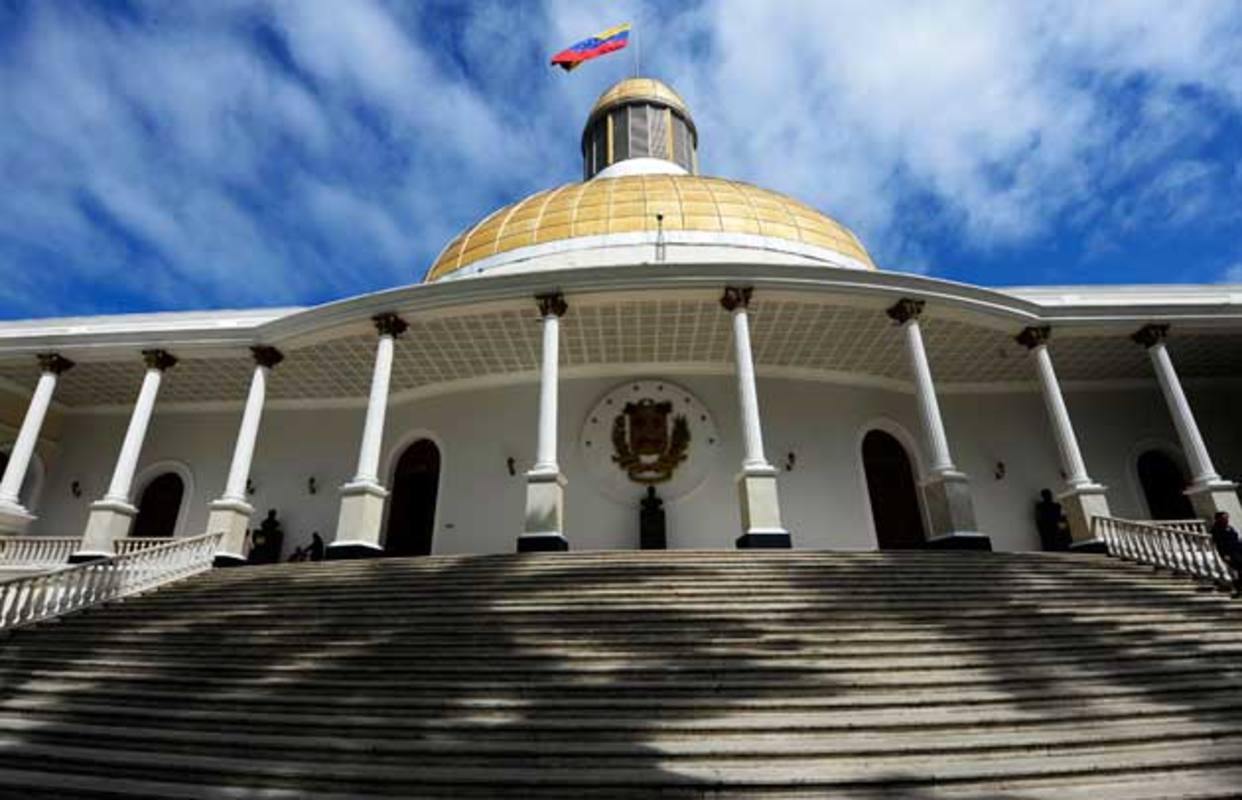
\includegraphics[width=300px]{39.jpg}%
\newline%
%
La Asamblea Nacional~aprobó en la plenaria de ayer, con los votos salvados de~la Fracción~16 de Julio y~La Causa R, un acuerdo mediante el cual declara inconstitucional la “pretensión del presidente Nicolás Maduro de continuar usurpando” el cargo a partir del 10 de enero de 2019, y llamó a los venezolanos y a la comunidad internacional a defender~la Constitución~y propiciar el cambio político en el país.%
\newline%
%
El Poder Legislativo también pidió a la comunidad internacional que “ante la tragedia sin precedentes” que vive Venezuela fortalezca su solidaridad con “las fuerzas democráticas” y mantenga, de manera efectiva y progresiva, “la presión legítima sobre el régimen”, con el fin de procurar una solución de la crisis y construir una transición democrática ordenada e inmediata.%
\newline%
%
Se comprometió a crear un marco normativo que asegure el cambio político, el retorno de la democracia y la reconciliación nacional, de acuerdo con~la Constitución~de 1999.%
\newline%
%
Los parlamentarios acordaron concertar, junto con la comunidad internacional, una solución política que posibilite la construcción, “sin venganza ni persecución, de un gobierno de paz para iniciar la transformación económica y social del país”. Además, que conduzca a la “atención urgente y eficaz de las necesidades socioeconómicas del pueblo, la liberación de todos los presos políticos, retorno de los exiliados y levantamiento de inhabilitaciones”.%
\newline%
%
En el acuerdo se señala que la solución debe llevar al restablecimiento de las competencias del Parlamento y la renovación de los poderes públicos, la disolución de la asamblea nacional constituyente, y a condiciones electorales democráticas para que se celebren elecciones generales que garanticen el derecho de elegir de los venezolanos, con observación nacional e internacional calificada e independiente.%
\newline%
%
Juan Guaidó, jefe de~la Fracción~de~la Unidad~y miembro de Voluntad Popular, ~fue el encargado de presentar el proyecto. Resaltó que es menester del Legislativo buscar los mecanismos para concretar la materialización de los puntos expuestos para “abrir las compuertas de la vida democrática por la cual tanto se ha luchado”.%
\newline%
%
El diputado José Luis Pirela explicó que~la Fracción~16 de Julio salvó su voto en el debate porque “una transición con dictadores no puede tener carácter democrático”.%
\newline%
%
Américo De Grazia, de~La Causa R, declaró que detallarán en su momento las observaciones sobre el acuerdo, del que afirmó no tenían conocimiento. “La unidad se construye con confianza. Es un ejemplo de cooperación y comunicación, no podemos venir arreados sin conocer exactamente de qué y cómo se trata”.%
\newline%
%
Alfonso Marquina, diputado por Primero Justicia, aclaró que este documento histórico no pretende crear una negociación con un gobierno que busca recursos para ganar tiempo. “Ratificamos la necesidad de una salida política”, enfatizó.%
\newline%
%
\end{document}